%!TEX root=../../../main.tex

For implementing the annotation system, an extensible design was considered, in
which different classes of metadata are constructed using a minimal set of base
elements.  By accounting for the targeted use cases and standard formats, such
as OA, the minimal information set we reckoned necessary for any type of
annotation consists of:
\begin{enumerate}
  \item The target of the annotation (e.g., a document, a Web page, etc.)
  \item The content; we target mostly plain text, with possible markup
        (e.g., \LaTeX), other types, such as multimedia, being possible by
        extending the base models (see below).
  \item The author of the annotation
  \item Time stamp
  \item Permissions of the annotation; arguably, this could also be provided as
        an extension, but as access control is an important aspect of Invenio,
        we considered that all metadata should have restriction rules
        integrated. Public access can also be encoded using this parameter.
\end{enumerate}

Starting from this base, further models can be defined. For example, to allow
attaching external files, only a new field referencing such data needs to be
added. Extensions should also be possible by slightly modifying one of the base
fields; for example, while in the general case the target field is an IRI, for
annotations targeting specific locations in Invenio record documents,
supplementary information (e.g., page number) needs to also be supplied, in the
same manner OA uses constraints. The model is briefly summarised in Fig.
\ref{fig:datamodel}.

In terms of the system that should provide the annotation facilities, the
following components need to be considered:
\begin{itemize}
  \item Front-end annotation editor; this is presented to end-users,
        who should fill in the target and content fields, the other information
        being assumed. Different annotation models can implement different
        editors, in order to guide users into inputting complete and valid data.
  \item Annotation persistent storage.
  \item Annotation exporter; this should provide access to metadata to third
        parties, in a standardised format, and with regard to the access control
        policies.
\end{itemize}
Clearly, seamless communication between these components must be provided,
through an equivalent of the controller in the Model--View--Controller pattern.
Thus, the data flow of the annotation system can be summarised as in Fig.
\ref{fig:dataflow}.

One issue that needs to be considered regarding the extensible annotation model
regards the method used for data persistence. Invenio currently uses an SQL
database, and this model does not fit well the proposed definitions. For
example, if the three models in Fig. \ref{fig:datamodel} are considered, it can
be seen that certain difficulties in expressing them in relational terms will
be encountered. Using separate tables for each model is clearly not optimal in
terms of future scalability, while using one table by, for example, encoding
data in a free text field with a loose syntax, is difficult to maintain,
error-prone, and possibly sub-optimal in terms of system performance.

Fortunately, the new version of Invenio brings support for storing JSON
documents, and the project fully leveraged this possibility, as explained in the
next sections. Apart from solving the issue described above, this method also
facilitates distribution of annotation data to third parties, as JSON is widely
used on the Web for these purposes.

\begin{figure}[!ht]
  \centering
  \fbox{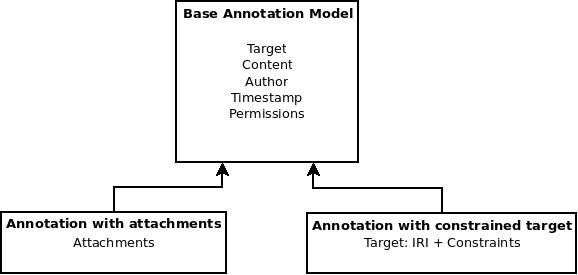
\includegraphics[scale=0.7]{static/dia/datamodel.jpeg}}
  \caption[Basic annotation data model]
          {Basic annotation data model. A series of base fields are defined,
           upon which various annotation types can build more complex
           structures, both by adding new fields or modifying existing ones.}
  \label{fig:datamodel}
\end{figure}

\begin{figure}[!ht]
  \centering
  \fbox{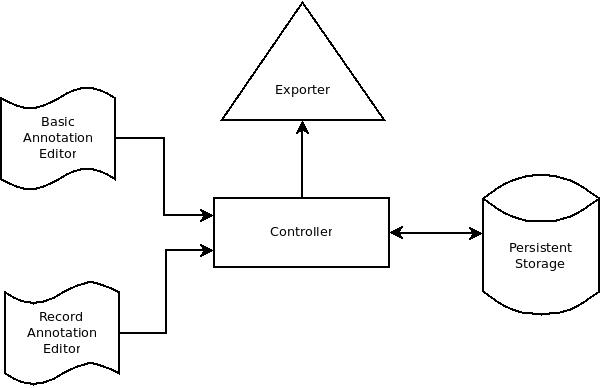
\includegraphics[scale=0.7]{static/dia/dataflow.jpeg}}
  \caption[Annotation system data flow]
          {Annotation system data flow. End-user create new annotations using
           the specialised editors, content being persisted in a database.
           Metadata can be publicised to interested third parties.}
  \label{fig:dataflow}
\end{figure}
